\twocolumn[\colorsection{Preguntas sobre magnetostática para el análisis}]
\textit{En esta sección se requiere brindar respuestas argumentadas.}
\setcounter{figure}{0}
%
\begin{Exercise}
    Explique si las siguientes afirmaciones son verdaderas o falsas:
    \begin{enumerate}[a)]
        \item La fuerza magnética que actúa sobre una partícula cargada móvil es siempre perpendicular a la velocidad de la partícula.
        \item El momento del par que actúa sobre un imán tiende a alinear el momento magnético en la dirección del campo magnético.
        \item Una espira de corriente en un campo magnético uniforme se comporta como un pequeño imán.
        \item El período de una partícula moviéndosa en círculo en un campo magnético es proporcional al radio del círculo.
        \item Los imanes existen en la naturaleza y presentan dos o más polos.
        \item Al igual que los cuerpos electrizados, los polos de distinto tipo de atraen y los de igual tipo se repelen.
    \end{enumerate}
\end{Exercise}
%
\begin{Exercise}\label{p:preguntas01}
    Contestar cuál opción es la correcta. Al hacer dos cortes en un imán de barra con dos polos en los extremos, dividiéndolo en tres partes iguales, como se muestra en la figura \ref{f:preguntas01}, se obtienen:
    \begin{enumerate}[a)]
        \item Tres imanes completos (cada uno con sus polos Norte y Sur).
        \item Uno con un polo Norte, uno con un polo Sur, y un fragmento no magnetizado.
        \item Dos imanes completos y un fragmento no magnetizado.
        \item Dos fragmentos no magnetizados y un imán completo.
        \item Tres fragmentos no magnetizados.
    \end{enumerate}
\end{Exercise}
%
\begin{center}
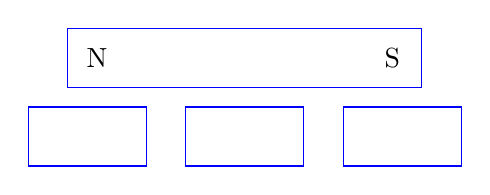
\begin{tikzpicture}[scale=0.5]
    \draw[blue] (0,0) rectangle (9,1.5);
    \draw[blue] (3,-2) rectangle (6,-0.5);
    \draw[blue] (-1,-2) rectangle (2,-0.5);
    \draw[blue] (7,-2) rectangle (10,-0.5);
    \draw[] (0.75,0.75) node [] {N};
    \draw[] (8.25,0.75) node [] {S};
\end{tikzpicture}
\captionof{figure}{Problema \ref{p:preguntas01}\label{f:preguntas01}}
\end{center}
%
\begin{Exercise}
    ¿Podría una partícula cargada moverse a través de un campo magnético sin experimentar fuerza alguna?
\end{Exercise}
%
\begin{Exercise}
    La fuerza magnética sobre una partícula cargada en movimiento siempre es perpendicular al campo magnético. ¿La trayectoria siempre es perpendicular a las líneas de campo magnético?
\end{Exercise}
%
\begin{Exercise}
    Una partícula cargada se mueve a través de una región del espacio con velocidad constante. Si el campo magnético externo es igual a cero en esta región, ¿se puede concluir que el campo eléctrico externo también vale cero? (Con ``externo'' nos referimos a aquellos campos que no son producidos por la partícula cargada.) Si el campo eléctrico externo es cero en la región, ¿se puede concluir que el campo magnético externo también es cero?
\end{Exercise}
%
\begin{Exercise}
    ¿Cómo puede determinarse la dirección de un campo magnético únicamente con observaciones cualitativas de la fuerza magnética sobre un alambre recto que transporta corriente?
\end{Exercise}
%
\begin{Exercise}
    Un estudiante afirma que si un relámpago cae sobre un mástil metálico, la fuerza ejercida por el campo magnético terrestre sobre la corriente en el mástil puede ser lo suficientemente grande como para doblarlo. Las corrientes comunes de los relámpagos son del orden de $10^4\,\text{A}$ a $10^5\,\text{A}$. ¿La opinión del estudiante está justificada?
\end{Exercise}
%
\begin{Exercise}
    Contestar verdadero o Falso (Si la afirmación es verdadera, explicar por qué lo es. Si es falsa, un contraejemplo).
    \begin{enumerate}[a)]
        \item El campo magnético debido a un elemento de corriente es paralelo a este elemento.
        \item El campo magnético producido por un elemento de corriente varía en razón inversa con el cuadrado de la distancia al elemento.
        \item El campo magnético debido a un conductor largo varía en razón inversa con el cuadrado de la distancia al conductor.
        \item La ley de Amp\`ere es válida sólo si existe alto grado de simetría.
    \end{enumerate}
\end{Exercise}
%
\begin{Exercise}
    ¿Qué opción es correcta? El magnetismo terrestre se debe principalmente
    \begin{enumerate}[a)]
        \item al movimiento de rotación de la Tierra en torno de su eje.
        \item al viento solar.
        \item al alto contenido de hierro del núcleo terrestre.
        \item a que el núcleo terrestre rota de un modo ligeramente diferente al resto del planeta.
        \item por las corrientes de lava volcánica que se mueve debajo de la corteza terrestre y sobre la cual flotan los continentes.
    \end{enumerate}
\end{Exercise}
%
\begin{Exercise}
    En los libros de texto se analiza el campo magnético de un conductor infinitamente largo y recto que transporta una corriente. Por supuesto, no hay nada que sea infinitamente largo. ¿Cómo determinaría usted que un alambre en particular es suficientemente largo como para considerarlo infinito?
\end{Exercise}
%
\begin{Exercise}
    Suponga que tiene tres alambres largos y paralelos dispuestos de manera que, vistos en sección
    transversal, se encuentran en los vértices de un triángulo equilátero. ¿Hay algún modo de arreglar las corrientes de manera que los tres alambres se atraigan entre sí? ¿Y de modo que los tres se rechacen entre sí?
\end{Exercise}
%
\begin{Exercise}
    Dos espiras circulares concéntricas coplanares de alambre, de distinto diámetro, conducen corrientes en el mismo sentido. Describa la naturaleza de la fuerza ejercida sobre la espira interior por la espira exterior, y sobre la espira exterior por la espira interior.
\end{Exercise}
%
\begin{Exercise}
    Se envió una corriente a través de un resorte helicoidal. El resorte se contrajo, como si se hubiera comprimido. ¿Por qué?
\end{Exercise}
%
\begin{Exercise}
    Si la magnitud del campo magnético a una distancia R de un alambre largo, recto y que conduce
    corriente es B, ¿a qué distancia del alambre el campo tendrá una magnitud de 3B?
\end{Exercise}
%
\begin{Exercise}
    Dos cables muy largos y paralelos, transportan corrientes iguales en sentidos opuestos. ¿Hay
    algún sitio en el que sus campos magnéticos se anulen por completo? Si es así, ¿dónde? Si no, ¿por qué? ¿Cómo cambiaría la respuesta si las corrientes tuvieran el mismo sentido?
\end{Exercise}
%
